% LaTeX source for ``การเรียนรู้ของเครื่องสำหรับเคมีควอนตัม (Machine Learning for Quantum Chemistry)''
% Copyright (c) 2022 รังสิมันต์ เกษแก้ว (Rangsiman Ketkaew).

% License: Creative Commons Attribution-NonCommercial-NoDerivatives 4.0 International (CC BY-NC-ND 4.0)
% https://creativecommons.org/licenses/by-nc-nd/4.0/

\chapter{ชุดข้อมูลทางเคมี}
\label{ch:chem_dataset}

%--------------------------
\section{ชุดข้อมูล}
\label{sec:dataset}
%--------------------------

\begin{figure}[H]
    \centering
    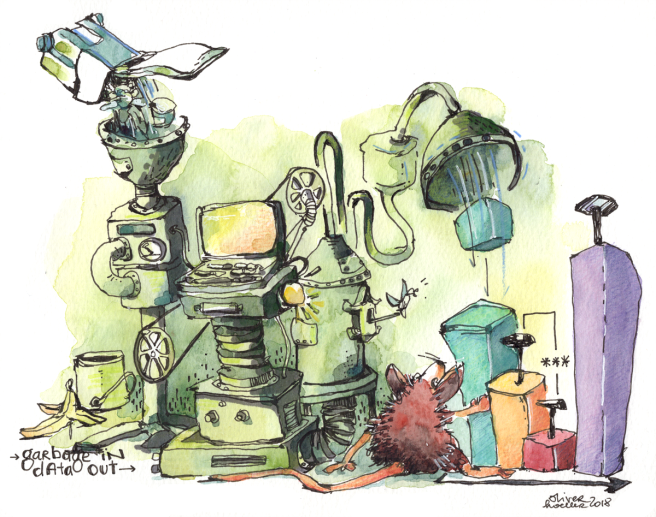
\includegraphics[width=0.75\linewidth]{fig/gigo.png}
    \caption{แนวคิดของ Garbage In, Garbage Out (GIGO) (เครดิตภาพ: \url{http://oliverhoeller.com})}
    \label{fig:gigo}
\end{figure}

ชุดข้อมูล (Data Set) คือการเก็บข้อมูลให้อยู่ในรูปแบบที่สามารถแบ่งประเภทของข้อมูลในชุดข้อมูลได้ โดยส่วนใหญ่แล้วเรามักจะเก็บข้อมูลในรูปแบบของตาราง โดยตารางของชุดข้อมูลนั้นอาจจะมีหลายคอลัมน์ก็ได้ โดยแต่ละคอลัมน์จะแสดงถึงตัวแปรเฉพาะของข้อมูล ข้อมูลนั้นเป็นสิ่งที่สำคัญและเป็นองค์ประกอบที่ขาดไม่ได้เลยในการสร้างโมเดลปัญญาประดิษฐ์ ซึ่งการที่เรามีข้อมูลมหาศาลในทุกวันนี้ก็อาจจะเรียกได้ว่าเป็นสาเหตุหลักที่ทำให้เกิด ML ขึ้นมาได้ ชุดข้อมูลถือได้ว่าเป็นหัวใจสำคัญของ ML เลยก็ว่าได้ ถ้าหากเรามีชุดข้อมูลที่มีคุณภาพดี เราก็จะสามารถสร้าง Feature Input Vector ที่มีคุณภาพให้กับโมเดลต้องการฝึกสอนได้ แต่ถ้าหากชุดข้อมูลของเราไม่ดี สิ่งที่ตามมาก็คือโมเดลที่ถูกฝึกสอนออกมานั้นก็จะมีประสิทธิภาพในการทำนายที่ต่ำมาก (Garbage In, Garbage Out) 

\idxboth{ชุดข้อมูล}{Dataset}
\idxboth{ขยะเข้า ขยะเข้า}{Garbage In, Garbage Out}

\begin{figure}[H]
    \centering
    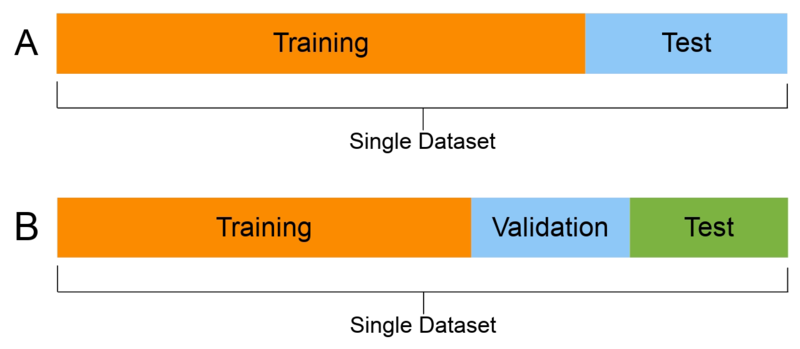
\includegraphics[width=0.7\linewidth]{fig/dataset.png}
    \caption{ตัวอย่างชุดข้อมูลแบบ 2 มิติ โดยมี Feature คือ Score, Attempts, และ Qualify (เครดิตภาพ: w3resource.com)}
    \label{fig:dataset}
\end{figure}

เรามาดูรายละเอียดของชุดข้อมูลกันมากกว่านี้ดีกว่าครับ เริ่มจากเราต้องทำความเข้าใจมิติของชุดข้อมูล (Dimensionality of Dataset) กันก่อน ซึ่งมิติของชุดข้อมูลก็จะมีตั้งแต่ 1 มิติ, 2 มิติ, 3 มิติ, 4 มิติ หรือสูงมากกว่านั้นก็ได้ ให้ลองนึกถึง Tensor ซึ่งเราสามารถเพิ่มจำนวนมิติของข้อมูลได้ สำหรับกรณีที่ชุดข้อมูลมี 1 มิตินั้นจะง่ายที่สุดเพราะเราจะมองว่าชุดข้อมูลแบบนี้เป็นเวกเตอร์ก็ได้ ชุดข้อมูล 1 มิติก็คือข้อมูลที่มีหลายแถวแต่มีแค่ 1 หลัก หรือจะเป็นชุดข้อมูลที่มีเพียงแค่ 1 แถวแต่มีหลายหลักก็ได้ สำหรับชุดข้อมูลแบบ 2 มิตินั้นให้เปรียบเทียบกับตาราง ซึ่งตารางประกอบไปด้วยแถวและหลัก โดยเราจะมองว่าตารางนั้นจริง ๆ แล้วก็คือเมทริกซ์ก็ได้ ซึ่งชุดข้อมูล 2D ประกอบด้วยมิติของแถว (Row) และมิติของหลักหรือคอลัมน์ (Column) เมื่อนำจำนวนของแถวคูณกับจำนวนของหลัก (Row x Column) จะได้ขนาดของชุดข้อมูล (Size) ซึ่งสอดคล้องกับขนาดของเมทริกซ์ เช่น ชุดข้อมูลขนาด 125 x 50 หมายความว่าชุดข้อมูลนี้คือชุดข้อมูลขนาด 2 มิติ ที่มีจำนวนข้อมูลทั้งหมด 125 แถว แต่ละแถวมี 50 หลัก สำหรับชุดข้อมูล 3 มิติ ก็จะมีอีก 1 มิติเพิ่มเข้ามานอกเหนือจากแถวกับหลักซึ่งจะถูกเรียกว่าอะไรนั้นก็ขึ้นอยู่กับว่าข้อมูลนั้นเป็นข้อมูลประเภทไหน เพราะว่าบางครั้งเราก็ไม่ได้ใช้คำว่าแถวกับหลัก เช่น ถ้าเป็นชุดข้อมูลรูปภาพ ก็จะใช้ ความสูง x ความกว้าง x ความลึก (Height x Width x Depth) ซึ่งก็สามารถเรียงสลับได้
\idxth{ชุดข้อมูล!มิติของชุดข้อมูล}
\idxen{Dataset!Dimensionality of Dataset}

โดยชุดข้อมูลพื้นฐานที่ใช้กันอย่างแพร่หลายทางด้าน ML ได้แก่ชุดข้อมูลดอกไม้ (Iris Dataset) กับชุดข้อมูลลายมือตัวเลขอารบิก (MNIST Dataset)

%--------------------------
\section{ประเภทและการแบ่งชุดข้อมูล}
\label{sec:split_dataset}
\idxth{ชุดข้อมูล!ประเภทของชุดข้อมูล}
\idxen{Dataset!Type of Dataset}
\idxth{ชุดข้อมูล!การแบ่งชุดข้อมูล}
\idxen{Dataset!Dataset Splitting}
%--------------------------

ชุดข้อมูลที่ใช้ใน ML นั้นโดยทั่วไปแล้วมักจะมีอยู่ 2 ประเภทคือชุดข้อมูลสำหรับการฝึกสอน (Training Set) และชุดข้อมูลสำหรับการทดสอบ (Test Set) ซึ่งวัตถุประสงค์ของชุดข้อมูลทั้งสองประเภทนี้ก็ตรงตัวเลยก็คือ Training Set จะถูกนำมาใช้ในการฝึกสอนโมเดล ส่วน Test Set จะถูกเก็บไว้ใช้ในการทดสอบโมเดลหรือการทำนายคำตอบที่โมเดลถูกสอนมา (Prediction) อย่างไรก็ตาม การฝึกสอนโมเดลโดยการใช้ Train Set ทั้งหมดนั้นมักจะทำให้เกิดความโน้มเอียง (Bias) ที่เกิดขึ้นจากชุดข้อมูลและส่งผลให้เกิด Biased ในขั้นตอน Prediction ด้วย เพราะป้องกันเหตุการณ์ดังกล่าวและทำให้เกิด Bias น้อยที่สุด เรามักจะทำการแบ่ง (Split) ชุดข้อมูลฝึกสอนให้เป็นชุดข้อมูลสำหรับการฝึกสอนจริง ๆ (Actual Training Set) และชุดข้อมูลสำหรับการตรวจสอบและยืนยันความถูกต้องซึ่งเรียกอีกอย่างว่า Validation Set

\begin{figure}[H]
    \centering
    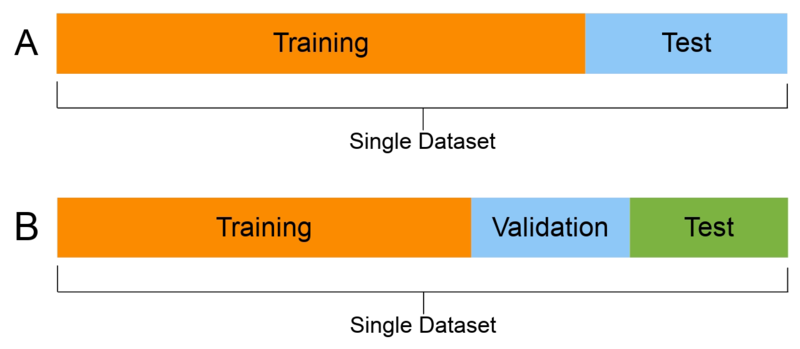
\includegraphics[width=0.8\linewidth]{fig/dataset_splitting.png}
    \caption{การแบ่งชุดข้อมูลทั้งหมดออกเป็น (A) Training Set และ Test Set และ (B) Training Set, Validation Set และ 
    Test Set (เครดิตภาพ: Wikimedia Commons)}
    \label{fig:dataset_splitting}
\end{figure}

ภาพที่ \ref{fig:dataset_splitting} แสดงสัดส่วนแบบคร่าว ๆ ในการแบ่งชุดข้อมูลหลักออกเป็น Training Set และ Test Set และแสดงการแบ่งชุดข้อมูล Training Set อีกครั้งให้เป็น Actual Training Set ที่จะถูกนำไปใช้ในการฝึกสอนโมเดลจริง ๆ และ Validation Set ที่จะถูกนำมาทดสอบโมเดลเพื่อเป็นการหยั่งเชิงความสามารถของโมเดลก่อนที่จะนำไปใช้ทำนายค่าของเอาต์พุตของข้อมูลใน Test Set โดยทั่วไปแล้วหลาย ๆ คนมักจะทำการแบ่งชุดข้อมูลโดยใช้อัตราส่วนคือ 80\% (สำหรับ Training Set) และ 20\% (สำหรับ Test Set) ตามหลักการของ Pareto\footnote{\url{https://en.wikipedia.org/wiki/Pareto_principle}}

แล้วขั้นตอนการลด Bias นั่นมันเกิดขึ้นได้อย่างไร คำตอบก็คือในการแบ่งข้อมูลออกมาเป็น Validation Set (เช่นแบ่งออกมา 20\% จากทั้งหมด) โดยทำการสุ่มเลือกบางส่วนของข้อมูลออกมา ซึ่งถ้าหากเราทำวนไปแบบนี้ไปเรื่อย ๆ เราจะเรียกว่าเป็นการทำ Validation แบบข้ามไปมาทั่วทั้ง Training Set ซึ่งเมื่อเรานำ Training Set แต่ละชุดไปฝึกสอนโมเดล เราจะได้ประสิทธิภาพของโมเดลแบบเฉลี่ย เปรียบเสมือนเป็นการเกลี่ยหาความเท่ากันของข้อมูลนั่นเอง (กระจายออกไปให้เสมอกัน) ท้ายที่สุดแล้วถ้าเราแบ่งชุดข้อมูลตามที่ได้อธิบายมา เราจะมีอัตราส่วนของชุดข้อมูลย่อย ๆ แต่ละประเภท ดังนี้
%
\begin{itemize}[topsep=0pt,noitemsep]\setlength\itemsep{0.5em}
    \item Training: 80\%
    \begin{itemize}[topsep=0pt,noitemsep]\setlength\itemsep{0.5em}
        \item Actual Training Set: 60\%
        
        \item Cross Validation: 20\%
    \end{itemize}
    
    \item Testing: 20\%
\end{itemize}

นอกจากนี้แล้วเรายังสามารถแบ่งชุดข้อมูลตามประเภทของอัลกอริทึมของ ML ได้ด้วย โดยแบ่งออกตามประเภทของการเรียนรู้ ดังนี้
%
\begin{itemize}[topsep=0pt,noitemsep]\setlength\itemsep{0.5em}
    \item การเรียนรู้แบบมีผู้สอน : นำข้อมูลที่ใช้ในการฝึกสอนมาแยกประเภทผลลัพธ์ด้วยการติดป้ายกำกับ (Labels/Class) เป็นผลเฉลย จากนั้นนำข้อมูลที่ติดป้ายแล้วไปใช้ในการฝึกโมเดลที่ทำงานผ่านอัลกอริทึมสำหรับสร้างโมเดลที่ใช้ในการทำนายผลลัพธ์
    
    \item การเรียนรู้แบบไม่มีผู้สอน : ชุดข้อมูลสำหรับ ML ประเภทนี้จะเป็นแบบไม่ถูกจัดประเภทหรือติดป้ายกำกับข้อมูล วิธีนี้โมเดลของเราจะ    คาดเดาข้อมูลที่ได้รับและทำความเข้าใจถึงโครงสร้างที่ซ่อนอยู่แต่ไม่สามารถหาผลลัพธ์ที่ถูกต้องได้ 100\% แต่จะใช้วิธีสำรวจข้อมูลและใช้การ    ประมาณการว่าข้อมูลนั้นคืออะไร
\end{itemize}

%--------------------------
\section{การสร้างชุดข้อมูล}
\label{sec:create_dataset}
\idxth{ชุดข้อมูล!การสร้างชุดข้อมูล}
%--------------------------

\begin{figure}[H]
    \centering
    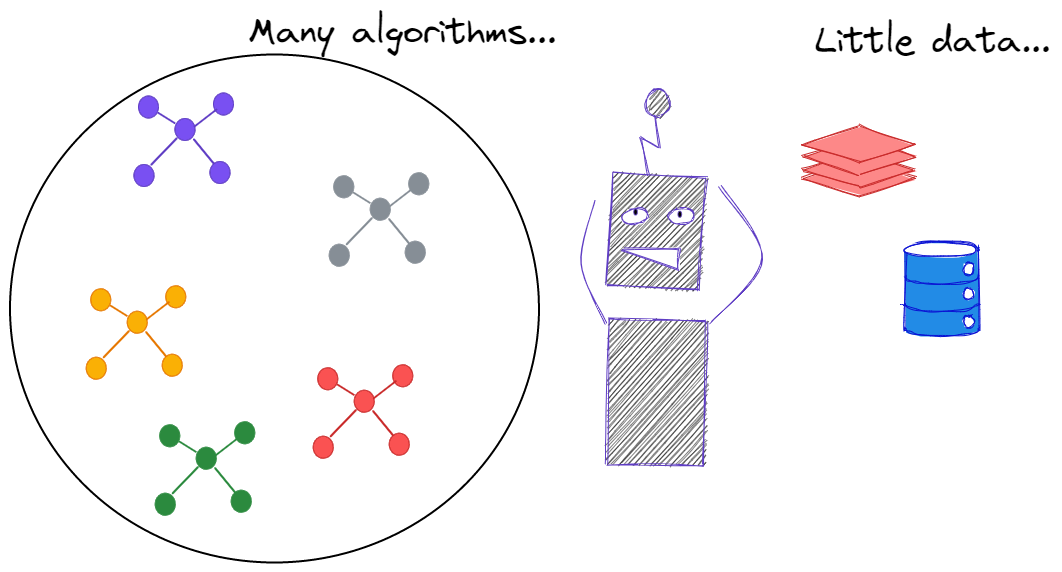
\includegraphics[width=0.8\linewidth]{fig/many_ml_little_dataset.png}
    \caption{แสดงปัญหาของการที่เรามีชุดข้อมูลที่มีขนาดเล็กเกินไป ซึ่งอัลกอริทึม ML ส่วนใหญ่นั้นต้องการชุดข้อมูลที่มีขนาดใหญ่ (เครดิตภาพ: \url{https://www.exxactcorp.com})}
    \label{fig:many_ml_little_dataset}
\end{figure}

โดยทั่วไปแล้วการเลือกใช้อัลกอริทึม ML นั้นควรจะต้องสอดคล้องกับขนาดของชุดข้อมูล (ปริมาณข้อมูล) ปัญหาก็คือว่าเรามีอัลกอริทึม ML ให้เลือกใช้เยอะมากแต่ว่าบางครั้งเรามีชุดข้อมูลที่มีขนาดเล็กมากหรือไม่มีชุดข้อมูลเลย ดังนั้นสิ่งที่เราต้องทำก็คือสร้างชุดข้อมูลขึ้นมาเองจากข้อมูลดิบหรือทำการเพิ่มปริมาณข้อมูลเพื่อให้ได้ชุดข้อมูลที่มีขนาดที่เหมาะสมเพราะว่าอัลกอริทึม ML หลาย ๆ อัลกอริทึมนั้นต้องการชุดข้อมูลที่มีขนาดใหญ่ ซึ่งถ้าถามว่าเราต้องการชุดข้อมูลที่ใหญ่ขนาดไหนนั้นไม่มีใครสามารถตอบได้ เพราะว่าชุดข้อมูลแต่ละประเภทนั้นไม่เหมือนกัน แต่ถ้าหากเรามีชุดข้อมูลที่ใหญ่ไว้ก่อนก็จะได้เปรียบ เพราะว่าการที่เรามีข้อมูลที่เยอะนั้นย่อมทำให้การฝึกสอนโมเดลนั้นเป็นไปอย่างมีประสิทธิภาพ ขั้นตอนการสร้างชุดข้อมูลประกอบไปด้วย 3 ขั้นหลักดังนี้

\paragraph{1. รวบรวมข้อมูล (Data Collection)} สิ่งแรกที่เราจะทำในการมองหา Dataset ก็คือแหล่งข้อมูลที่เราสามารถนำข้อมูลมาใช้ได้ ถ้าหากแหล่งข้อมูลไม่น่าเชื่อถือเราก็มักจะได้ชุดข้อมูลที่มีคุณภาพต่ำซึ่งอาจจะมีข้อผิดพลาดในชุดข้อมูลด้วยเช่นกัน เช่น ข้อมูลที่ถูกสร้างขึ้นมา (ข้อมูลปลอมหรือ Fake Data) 

\paragraph{2. ประมวลผลข้อมูลก่อน (Data Preprocessing)} หลักการสำคัญข้อหนึ่งของวิทยาศาสตร์ข้อมูลก็คือทำความสะอาดชุดข้อมูล (Data Cleaning) รวมไปถึงการทราบที่มาที่ไปและการทำความเข้าใจชุดข้อมูล เราต้องถามตัวเองก่อนว่าชุดข้อมูลที่เราสนใจนั้นเคยถูกใช้มาก่อนหน้านี้แล้วหรือยัง ถ้าหากว่ายังและเป็นชุดข้อมูลใหม่ เราควรจะต้องตั้งข้อสังเกตหรือสมมติฐานไว้ก่อนว่าชุดข้อมูลชุดนี้อาจจะมีข้อมูลที่ผิดปกติซ่อนอยู่ได้ หรืออาจจะมีข้อมูลที่ไม่ครบถ้วนขาดหายไป เราสามารถทำการประมวลผลชุดข้อมูลก่อนนำไปใช้งานจริงได้โดยการดูที่คุณภาพของ Features รวมไปถึง Bias ภายในชุดข้อมูล บางชุดข้อมูลมี Features เยอะมากแต่ว่ามี Bias เยอะมาก ๆ กับ Features เพียงแค่ 2-3 Features นอกจากนี้แล้วปริมาณของชุดข้อมูลก็มีผลด้วยเพราะว่าถ้าหากเรามีปริมาณข้อมูลที่น้อยเกินไปก็อาจจะเกิดปัญหา Overfitting ได้ในภายหลัง

\paragraph{3. การทำคำอธิบายประกอบ (Annotatation)} หลังจากทำความสะอาดข้อมูลเสร็จเรียบร้อยแล้วสิ่งที่เราควรจะต้องในลำดับต่อไปคือ Annotate นั่นคือเป็นการทำให้มั่นใจว่าข้อมูลของเรานั้นมันสามารถนำไปใช้ในการสอนเครื่องจักรเข้าใจได้ อธิบายง่าย ๆ คือทำให้คอมพิวเตอร์สามารถเรียนรู้จากข้อมูลได้ นั่นก็เพราะว่าเครื่องจักรไม่สามารถเข้าใจข้อมูลเหมือนอย่างที่มนุษย์เข้าใจ ดังนั้นเราควรจะต้องทำการเพิ่มคำอธิบายเชิงดิจิทัลให้กับข้อมูลนั่นก็คือการระบุค่าเฉพาะสำหรับข้อมูลนั้น ๆ หรือที่เรียกว่าการติดป้าย (Labeling)

%--------------------------
\section{ปริภูมิเคมี}
\label{sec:chem_space}
\idxboth{ปริภูมิเคมี}{Chemical Space}
%--------------------------

\begin{figure}[H]
    \centering
    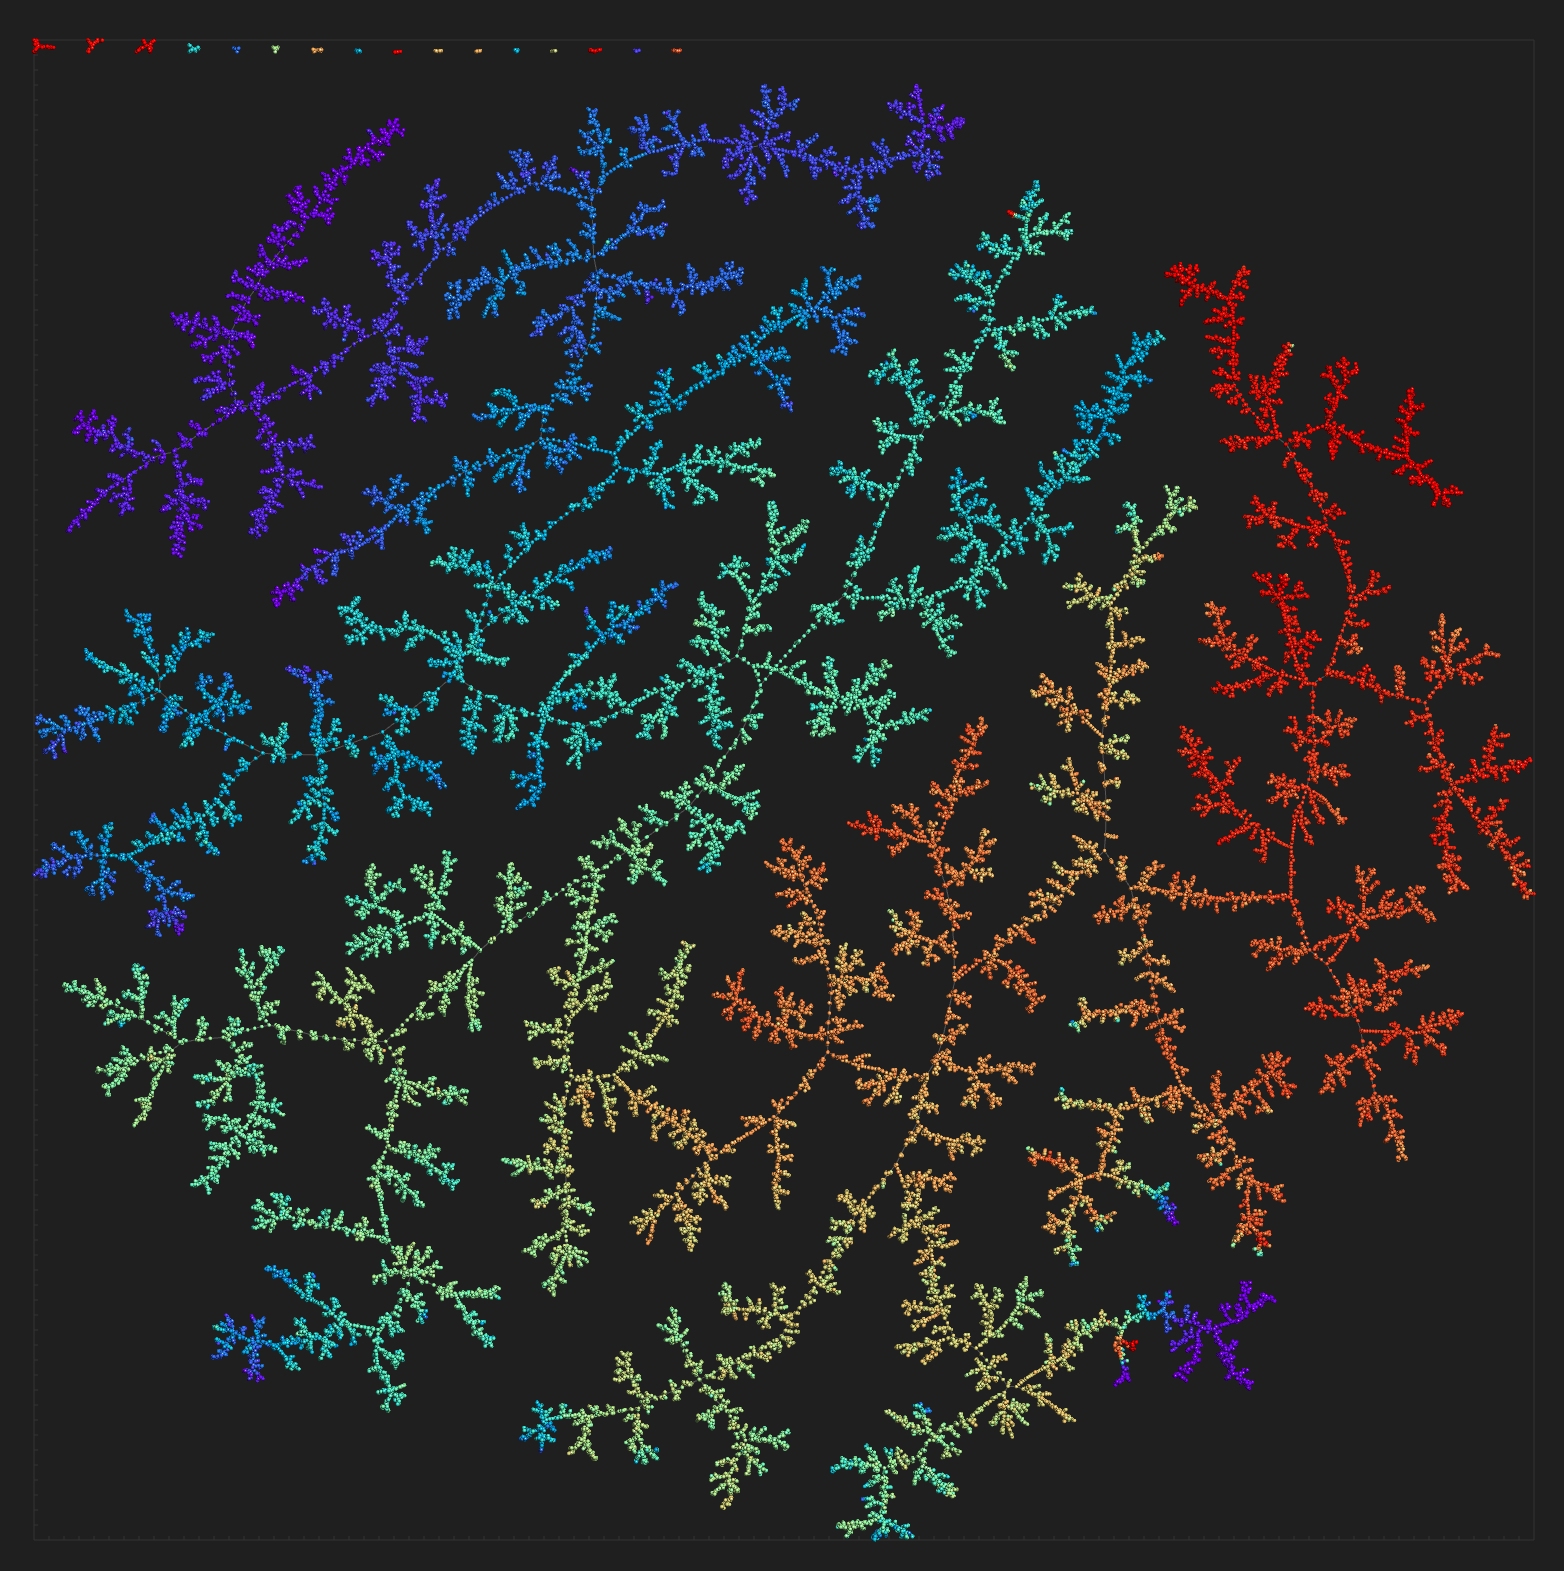
\includegraphics[width=0.8\linewidth]{fig/tmap_pdb.png}
    \caption{ปริภูมิเคมีของชุดข้อมูลโปรตีน Protein Data Bank (PDB) โดยใช้ไลบรารี่ TMAP ในการคำนวณหาความเชื่อมโยง}
    \label{fig:tmap_pdb}
\end{figure}

ปริภูมิเคมี (Chemical Space)\autocite{kirkpatrick2004} เป็นแนวคิดที่อธิบายว่าจำนวนและชนิดของโมเลกุลนั้นไม่ที่สิ้นสุด (Infinity) ซึ่งเปรียบเสมือนจำนวนดวงดาวในจักรวาลที่ก็ไม่มีที่สิ้นสุดเหมือนกัน ในขณะที่นักดาราศาสตร์พยายามสำรวจค้นหาดาวดวงใหม่นั้น นักเคมีก็สำรวจหาโมเลกุลชนิดใหม่ที่ซ่อนอยู่ในปริภูมิเคมี การค้นพบโมเลกุลใหม่นั้นอาจนำมาซึ่งคุณสมบัติเชิงเคมีที่น่าสนใจที่เราสามารถนำเอาองค์ความรู้ไปพัฒนาและต่อยอดในการศึกษาเคมีแขนงต่าง ๆ ได้ เช่น นำโมเลกุลที่ค้นพบใหม่นี้ไปศึกษาปฏิกิริยาใหม่ ๆ หรือรวมไปถึงการนำไปใช้ประโยชน์ในระยะยาวและใช้จริงในระดับอุตสาหกรรม เช่น การพัฒนาวัสดุหรือผลิตภัณฑ์ชนิดใหม่ 
\idxth{ชุดข้อมูลเคมีควอนตัม}
\idxen{Quantum Chemistry Dataset}

ภาพที่ \ref{fig:tmap_pdb} แสดงปริภูมิเคมีของชุดข้อมูล Protein Data Bank (PDB) ซึ่งเป็นชุดข้อมูลที่มีตำแหน่งของอะตอมของโปรตีน ข้อมูลที่เกี่ยวข้องกับโครงสร้างและข้อมูลที่เกี่ยวกับ NMR\footnote{ดูรายละเอียดของ PDB ได้ที่ \url{https://www.rcsb.org/}} โดยปริภูมินี้ถูกคำนวณด้วยวิธี Tree MAP (TMAP)\autocite{probst2020} ซึ่งเป็นการจัดเรียงและอธิบายความสัมพันธ์ระหว่างข้อมูลแต่ละจุดในรูปแบบของแผนภาพต้นไม้

\begin{figure}[H]
    \centering
    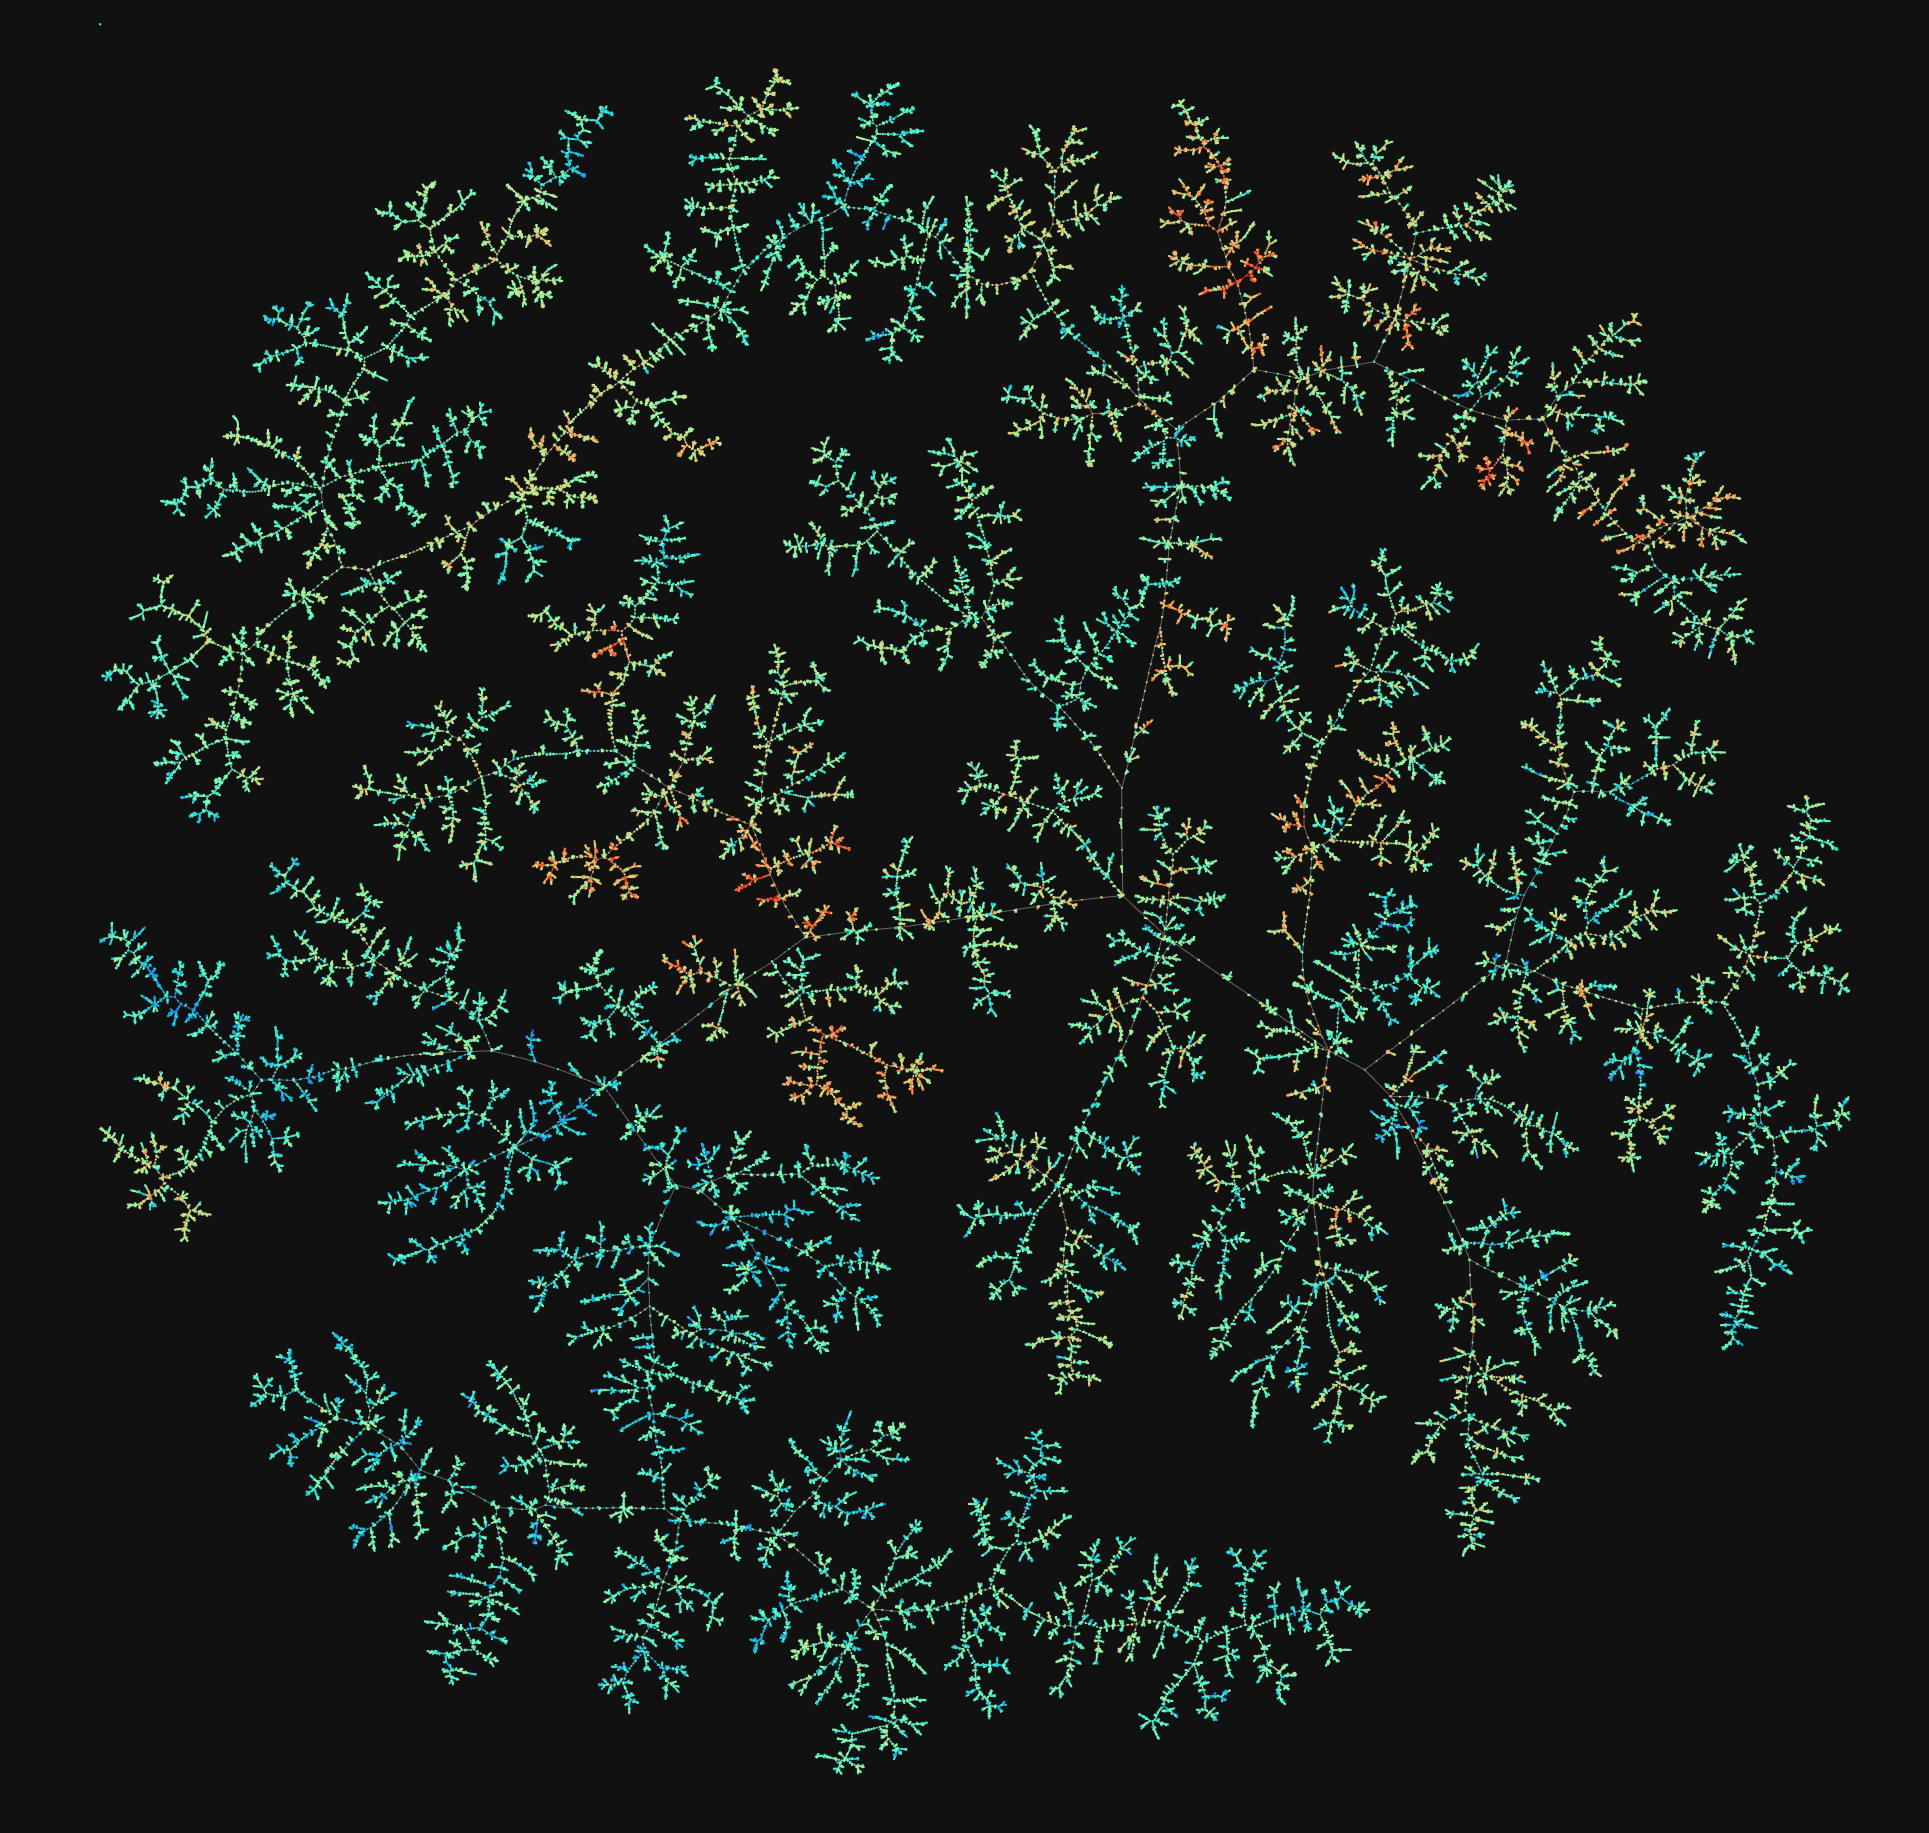
\includegraphics[width=0.8\linewidth]{fig/tmap_qm9.png}
    \caption{ปริภูมิเคมีของชุดข้อมูลโมเลกุลขนาดเล็ก QM9 โดยใช้ไลบรารี่ TMAP ในการคำนวณหาความเชื่อมโยง}
    \label{fig:tmap_qm9}
\end{figure}

\begin{figure}[H]
    \centering
    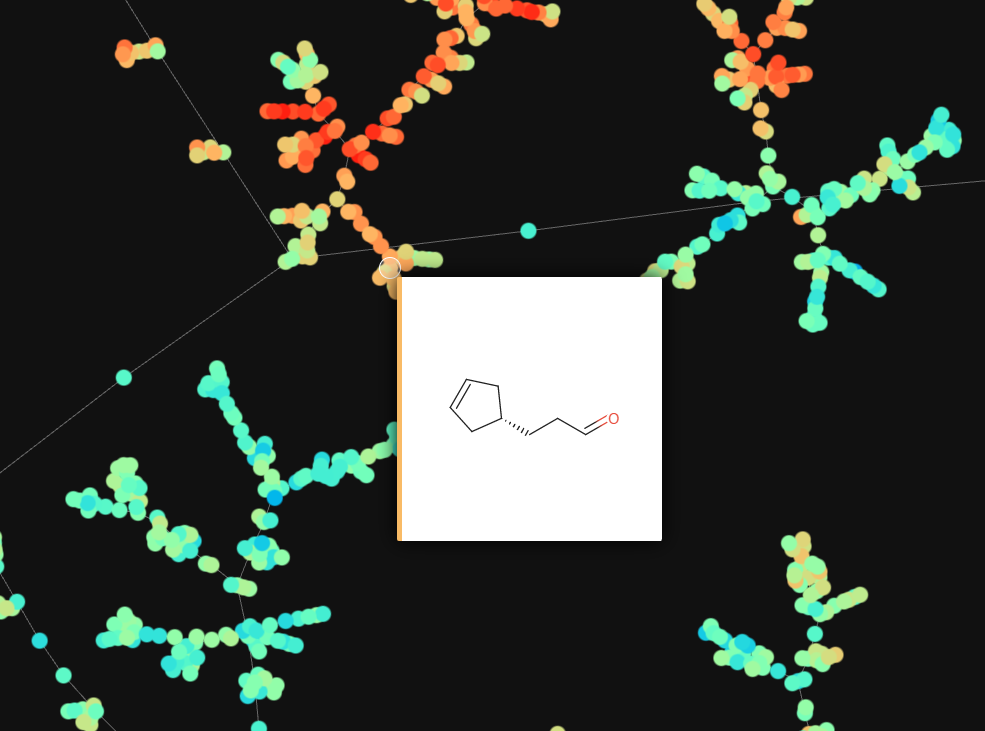
\includegraphics[width=0.8\linewidth]{fig/tmap_qm9_zoom.png}
    \caption{ภาพขยายของโมเลกุลที่สุ่มเลือกจากปริภูมิเคมีของชุดข้อมูลโมเลกุลขนาดเล็ก QM9}
    \label{fig:tmap_qm9_zoom}
\end{figure}

นอกจากนี้ยังมีอีกหนึ่งตัวอย่างนั่นคือปริภูมิเคมีของชุดข้อมูล QM9 ซึ่งแสดงในภาพที่ \ref{fig:tmap_qm9} ถ้าเราขยายเข้าไปใกล้ ๆ จะพบว่าจุดแต่ละจุดนั้นคือโมเลกุล เช่น โมเลกุลที่แสดงในภาพที่ \ref{fig:tmap_qm9_zoom} โดยเราสามารถตีความแผนภาพนี้ได้ว่ายิ่งจุดอยู่ใกล้กันมากเท่าไหร่ก็หมายความว่าโมเลกุลเหล่านั้นมีความเชื่อมโยงกันมากเท่านั้น และถ้าอยู่ห่างกัน เช่น อยู่กันคนละกลุ่ม ก็หมายความว่าโมเลกุลมีความสัมพันธ์กันน้อย สำหรับสีที่ใช้ในการไฮไลท์จุดแต่ละจุดนั้นแสดงถึงค่าของ cLogP ซึ่งเป็นสเกลที่บอกถึงความสามารถในการละลายนำซึ่งก็คือชอบน้ำ (Hydrophilic) หรือไม่ชอบน้ำ (Hydrophobic) นั่นเองซึ่งมีค่าตั้งแต่ -3.16 ถึง 3.76 และเป็นปริมาณที่ไม่มีหน่วย (Unitless)

%--------------------------
\section{การสร้างชุดข้อมูลเคมีควอนตัม}
\label{ssec:step_create_qm_dataset}
\idxth{ชุดข้อมูลเคมีควอนตัม!การสร้างชุดข้อมูล}
\idxen{Quantum Chemistry Dataset!Create Dataset}
%--------------------------

การสร้างชุดข้อมูลเคมีควอนตัมสามารถแบ่งออกได้เป็น 2 ประเภท ดังนี้

\begin{enumerate}[topsep=0pt]
    \item ชุดข้อมูลแบบที่มีเพียงหนึ่งโมเลกุลแต่มีหลาย Configuration: เป็นชุดข้อมูลที่โมเลกุลเพียงแค่หนึ่งโมเลกุลนั้นมีการจัดรูปแบบเชิงโครงสร้างที่หลากหลายแตกต่างกัน โดยเราสามารถใช้การจำลองด้วยวิธี Molecular Dynamics แล้วนำ Trajectory มาใช้เป็นชุดข้อมูล    ก็ได้ นอกจากนี้เรายังสามารถนำ Configuration (หรือจะเรียกว่า Conformer ก็ได้) ซึ่งเป็นโครงสร้างใน Trajectory มาคำนวณหา    คุณสมบัติเชิงอิเล็กทรอนิกส์เพิ่มเติมด้วยวิธีการคำนวณที่มีความแม่นยำมากกว่า เช่น DFT หรือ MP2

    \item ชุดข้อมูลแบบที่มีหลายโมเลกุล โดยแต่ละโมเลกุลมีเพียงหนึ่ง Configuration: ชุดข้อมูลแบบนี้จะมีความซับซ้อนในการสร้างที่มากกว่าชุดข้อมูลแบบแรกนั่นก็เพราะว่าเราจะต้องมีการสร้างอัลกอริทึมที่สามารถสร้างโมเลกุลที่มีความหลากหลายแตกต่างกันได้และโมเลกุลที่สร้าง    ขึ้นมานั้นจะต้องเป็นโมเลกุลที่เหมาะสม มีโครงสร้างที่เหมาะสม แต่ถูกต้องตามหลักเคมี เช่น มีจำนวนพันธะที่เหมาะสม สามารถนำมาสังเคราะห์    หรือศึกษาได้ในเชิงการทดลอง
\end{enumerate}

%--------------------------
\section{ชุดข้อมูลเคมีควอนตัมมาตรฐาน}
\label{sec:std_dataset}
\idxth{ชุดข้อมูลเคมีควอนตัม!ชุดข้อมูลเคมีมาตรฐาน}
\idxen{Quantum Chemistry Dataset!Standard Dataset}
%--------------------------

QM9 เป็นหนึ่งในชุดข้อมูลเคมีควอนตัมที่ได้รับความนิยมและถูกนำมาใช้ในงานวิจัย ML สำหรับเคมีควอนตัมเป็นอย่างมาก ซึ่งถูกใช้อย่างแพร่หลายตั้งแต่ปี ค.ศ. 2014 เป็นต้นมา\autocite{ruddigkeit2012,ramakrishnan2014} โดยบทความงานวิจัยแรกที่นำ QM9 มาใช้ในการทดสอบประสิทธิภาพของโมเดล ML นั้นได้รายงานค่าความผิดพลาดของโมเดล ML ที่ใช้ในการทดสอบว่ามีค่าคลาดเคลื่อนไม่เกิน 10 kcal/mol ซึ่งในเชิงการวัดนั้นถือว่ามีคลาดเคลื่อนที่เยอะมาก ๆ และในเวลาต่อมาก็ได้มีการพัฒนาระเบียบวิธีวิจัยรวมไปถึงโมเดล ML และ Descriptor ใหม่ ๆ จนทำให้ในปัจจุบันนั้นนักวิจัยสามารถที่จะทำนายหรือพยากรณ์ค่าพลังงานของโมเลกุลทางเคมีอินทรีย์ขนาดเล็กได้แม่นยำมากโดยมีค่าความคลาดเคลื่อนประมาณ 1 kcal/mol หรือต่ำกว่านั้น ซึ่งค่า 1 kcal/mol นี้ถือได้ว่าเป็น \textit{ค่าความถูกต้องทางเคมี (Chemical Accuracy)} ซึ่งเป็นค่ามาตรฐานที่ต่ำที่สุดที่เทคนิคทางการทดลองสามารถวัดได้ โดยถ้าหากค่าความคลาดเคลื่อนทางการคำนวณที่ต่ำไปกว่า 1 kcal/mol แล้วเทคนิคต่าง ๆ ในเชิงการทดลองจะไม่สามารถระบุความแตกต่างของความคลาดเคลื่อนที่แม่นยำได้อีกต่อไป

\begin{figure}[H]
    \centering
    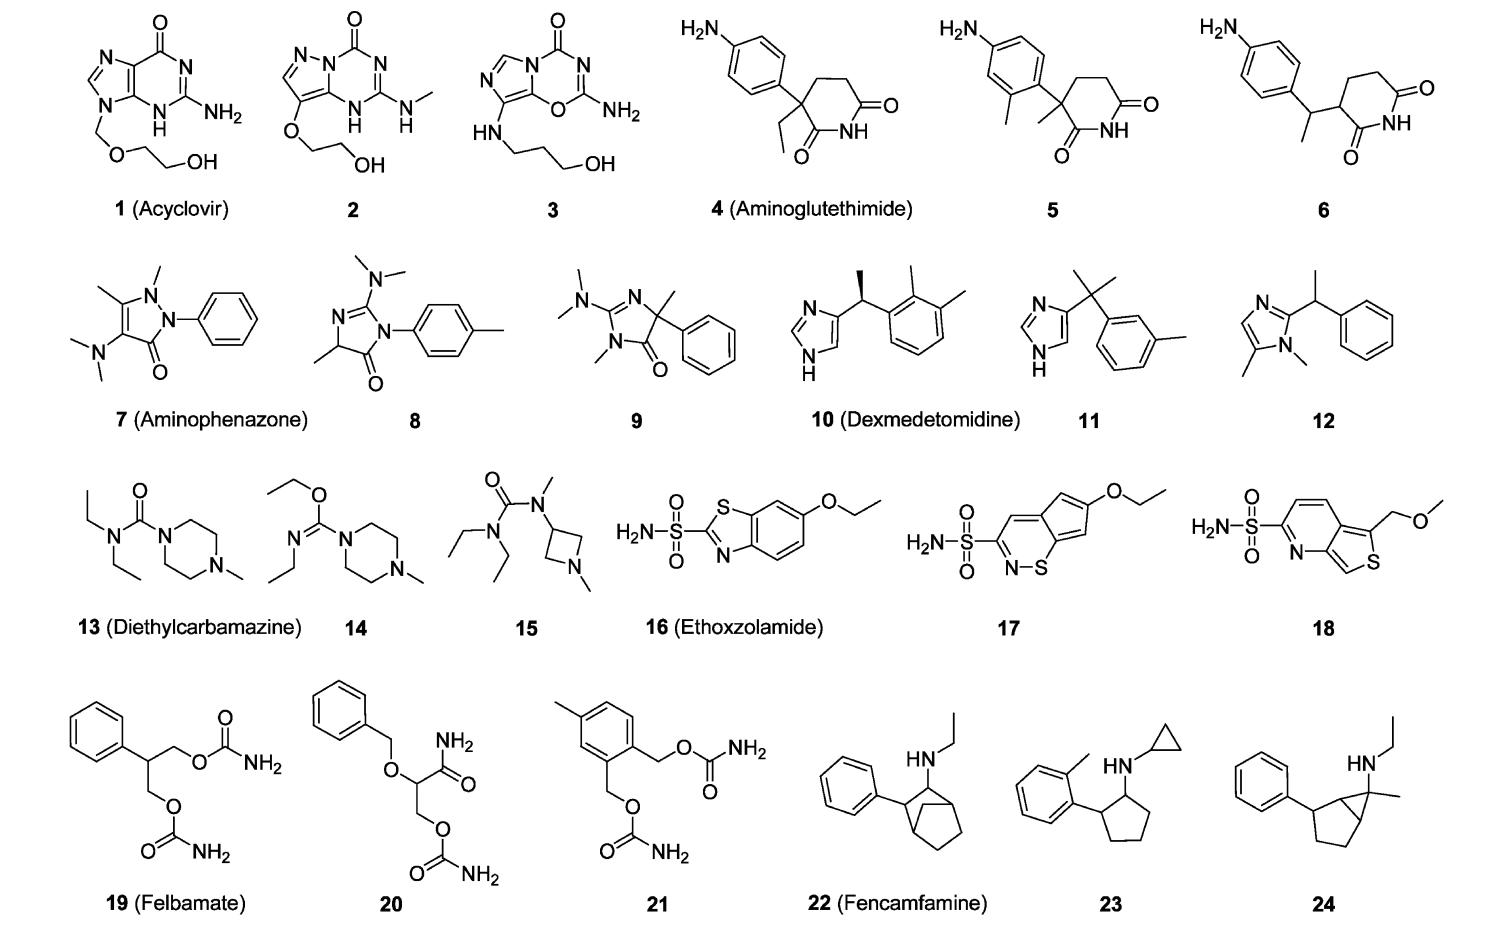
\includegraphics[width=\linewidth]{fig/qm9_molecules.jpg}
    \caption{โมเลกุลเพียงบางส่วนของชุดข้อมูล QM9}
    \label{fig:m9_mol}
\end{figure}

\begin{table}[H]
    \centering
    \caption{ข้อมูล Feature ของชุดข้อมูล QM9}
    \label{tab:qm9_feature}
    \small
    \begin{tabular}{llll}\toprule
    \textbf{ดัชนี} &\textbf{ชื่อ} &\textbf{หน่วย} &\textbf{คำอธิบาย} \\\midrule
    0 &index &- &Consecutive, 1-based Integer Identifier of Molecule \\
    1 &A &GHz &ค่าคงที่การหมุน (Rotational Constant) A \\
    2 &B &GHz &ค่าคงที่การหมุน (Rotational Constant) B \\
    3 &C &GHz &ค่าคงที่การหมุน (Rotational Constant) C \\
    4 &mu &Debye &ไดโพลโมเมนต์ (Dipole Moment) \\
    5 &alpha &Bohr$^3$ &Isotropic Polarizability \\
    6 &homo &Hartree &พลังงานของ Highest Occupied Molecular Orbital (HOMO) \\
    7 &lumo &Hartree &พลังงานของ Lowest Unoccupied Molecular Orbital (LUMO) \\
    8 &gap &Hartree &พลังงานระหว่าง LUMO and HOMO (Energy Gap) \\
    9 &r2 &Bohr$^2$ &Electronic Spatial Extent \\
    10 &zpve &Hartree &Zero Point Vibrational Energy \\
    11 &U0 &Hartree &พลังงานภายใน (Internal Energy) ที่ 0 K \\
    12 &U &Hartree &พลังงานภายใน (Internal Energy) ที่ 298.15 K \\
    13 &H &Hartree &Enthalpy at 298.15 K \\
    14 &G &Hartree &พลังงานอิสระ (Free Energy) ที่ 298.15 K \\
    15 &Cv &cal/(mol K) &ความจุความร้อน (Heat Capacity) ที่ 298.15 K \\
    \bottomrule
    \end{tabular}
\end{table}

QM9 ประกอบไปด้วยข้อมูลคุณสมบัติอิเล็กทรอนิกส์ของโมเลกุลมากถึง 134,000 โมเลกุล โดยภาพที่ \ref{fig:m9_mol} แสดงตัวอย่างของโมเลกุลเพียงบางส่วนของ QM9 ซึ่งทุกโมเลกุลในชุดข้อมูลนั้นมีธาตุพื้นฐานเป็นองค์ประกอบ ประกอบไปด้วย คาร์บอน (C), ไนโตรเจน, (N), ออกซิเจน (O), ไฮโดรเจน (H), และฟลูออรีน (F) โดย Feature หลักของ QM9 ก็จะมีพิกัดคาร์ทีเซียนของอะตอมทุกอะตอมในโมเลกุลซึ่งได้มาจากการคำนวณการปรับโครงสร้าง (Geometry Optimization) ด้วยระเบียบวิธี B3LYP/6-31G(2df,p) กับ G4MP2 และนอกจากนี้ยังมีค่า Label หรือค่าที่ไว้ใช้ในการเปรียบเทียบการพยากรณ์ดังแสดงในตารางที่ \ref{tab:qm9_feature}\footnote{โมเดล ML ที่เหมาะสมสำหรับการฝึกสอนด้วย QM9 นั้นจะต้องไม่ขึ้นกับ Translation, Rotation และ Permutation}

ชุดข้อมูล QM9 มีข้อมูลพิกัดคาร์ทีเซียน (Cartesian Coordinates), ลักษณะเฉพาะ (Features), และค่าพลังงานซึ่งเป็น Target ของข้อมูล โดยผู้อ่านสามารถดาวน์โหลดมาใช้งานได้ฟรีจากเว็บไซต์ \url{http://quantum-machine.org/datasets/} คราวนี้เราลองมาดูโค้ดสำหรับการใช้งาน QM9 โดยใช้ภาษา Python ตามด้านล่างนี้ได้เลย

\noindent ทำการเรียกใช้ไลบรารี่และอ่านไฟล์ของชุดข้อมูล

\begin{lstlisting}[style=MyPython]
# Import libraries
import ase.io as aio
import pandas as pd

# Read qm9.csv
qm9_data = pd.read_csv('./qm9.csv', index_col=0)
\end{lstlisting}

\vspace{1em}
\noindent เราสามารถใช้คำสั่งด้านล่างในการแสดง Target ได้

\begin{lstlisting}[style=MyPython]
# Convert energy from Hartree to kcal/mol
target = qm9_data['u0'] * 627.5096080305927 
print(target)

# Output
0         -25400.917498
40       -121896.331092
80       -146555.740566
120      -122481.233425
160      -168344.348805
              ...      
119800   -242900.012196
119840   -230424.279698
119880   -266202.856340
119920   -252980.566249
119960   -288738.466448
Name: u0, Length: 3000, dtype: float64
\end{lstlisting}

\vspace{1em}
\noindent อ่านพิกัดคาร์ทีเซียนของโมเลกุล

\begin{lstlisting}[style=MyPython]
# We read xyz coorinates of all the molecules with ase aio.read tool
ase_mols = [aio.read('data/qm9/qm9_xyz/' + mol + '.xyz') for mol in qm9_data.mol_id]
\end{lstlisting}

\vspace{1em}
\noindent ตรวจสอบขนาดของโมเลกุลที่ใหญ่ที่สุดในชุดข้อมูล

\begin{lstlisting}[style=MyPython]
# Check the size of molecules in the dataset
size=[]
for mol in ase_mols:
    num = len(mol.get_atomic_numbers())
    size.append(num)
# Show maximum size of the molecule in the dataset
max(size)

# Output
27
\end{lstlisting}

\vspace{1em}

โดยโค้ดด้านบนที่เราใช้สำหรับการโหลดชุดข้อมูล QM9 นั้นเราจะนำไปใช้ต่อในบทที่ \ref{sec:pred_pot_ener} สำหรับการทำนายพลังงานศักย์พื้นผิว (Potential Energy Surface) ของโมเลกุลของชุดข้อมูล QM9

นอกจาก QM9 แล้วยังมีชุดข้อมูลอื่น ๆ ที่นักวิจัยมักจะนำมาใช้ในการฝึกสอนโมเดลและทำวิจัย เช่น 
%
\begin{itemize}[topsep=0pt,noitemsep]\setlength\itemsep{0.5em}
    \item QM7\autocite{blum2009,rupp2012} เป็นส่วนหนึ่งของชุดข้อมูล GDB-13 ซึ่งเป็นชุดข้อมูลที่มีโมเลกุลเคมีอินทรีย์เกือบหนึ่งพันล้านโมเลกุล โดยชุดข้อมูล QM7 ประกอบไปด้วยโมเลกุลที่มีจำนวนอะตอมรวมกันสูงสุดถึง 23 อะตอม โดย Feature ที่ชุดข้อมูลนี้มีคือ Coulomb Matrix และพลังงานการทำให้เป็นอะตอม (Atomization Energy)
    
    \item QM7b\autocite{blum2009,montavon2013} เป็นส่วนขยายของชุดข้อมูล QM7 สำหรับใช้กับโมเดล ML ที่เป็นแบบ Multitask Learning โดยมี Feature เช่น Polarizability, ค่าไอเกนของ HOMO และ LUMO, และพลังงานกระตุ้น
    
    \item QM8\autocite{ruddigkeit2012,ramakrishnan2015} เป็นชุดข้อมูลสำหรับการพัฒนาโมเดล ML สำหรับการเรียนรู้สเปกตรัมเชิงอิเล็กทรอนิกส์ของโมเลกุล โดยชุดข้อมูลนี้มี Feature คือพลังงานกระตุ้นที่ถูกคำนวณด้วยวิธี Second-order Approximate Coupled-cluster (CC2)
    
    \item ISO17\autocite{schutt2017,schutt2017a,ramakrishnan2014} เป็นชุดข้อมูลที่ถูกสร้างขึ้นโดยใช้การจำลอง MD ด้วยโปรแกรม Fritz-Haber Institute ab initio Simulation (FHI-aims) โดยมี Feature คือพลังงานและแรงของแต่ละโมเลกุล
\end{itemize}

\noindent ซึ่งก็จะมี Label สำหรับวัตถุประสงค์ในการฝึกสอนโมเดลในการเพิ่มความสามารถการพยากรณ์คุณสมบัติเคมีของโมเลกุลที่ต่างกันออกไป โดยตารางที่ \ref{tab:compare_qm_dataset} แสดงการเปรียบเทียบชุดข้อมูลเคมีควอนตัม

\begin{table}[H]
    \centering
    \caption{เปรียบเทียบชุดข้อมูลเคมีควอนตัม}
    \label{tab:compare_qm_dataset}
    \begin{tabular}{cccccc}
    \toprule
    \textbf{Dataset} &\textbf{Data Type} &\textbf{จำนวน Tasks} &\textbf{จำนวนโมเลกุล} 
    &\textbf{Rec-Split} &\textbf{Heavy Atoms} \\
    \midrule
    QM7 &SMILES, 3D Coordinates &1 &7,165 &Stratified &$\leq$7 \\
    QM7b &3D Coordinates &14 &7,211 &Random &$\leq$7 \\
    QM8 &SMILES, 3D Coordinates &12 &21,786 &Random &$\leq$8 \\
    QM9 &SMILES, 3D Coordinates &12 &133,885 &Random &$\leq$9 \\
    \bottomrule
    \end{tabular}
\end{table}

ชุดข้อมูลที่รายงานในตารางที่ \ref{tab:compare_qm_dataset} สามารถดาวน์โหลดมาใช้งานได้ฟรีจากเว็บไซต์ 
\url{http://quantum-machine.org/datasets} 

นอกจากนี้ยังมีชุดข้อมูลเคมีควอนตัมใหม่ ๆ อีกหลายชุดข้อมูลที่ได้ถูกสร้างขึ้นที่ถูกพัฒนาขึ้นมา โดยมีรายละเอียดของคุณสมบัติเชิงอิเล็กทรอนิกส์ของชุดข้อมูลแต่ละชุด ดังนี้
%
\begin{itemize}[topsep=0pt,noitemsep]\setlength\itemsep{0.5em}
    \item \textbf{ANI-1}\autocite{smith2017a} DFT: Total Energy
    
    \item \textbf{QMugs}\autocite{mendez2019} 
    \begin{itemize}[topsep=0pt,noitemsep]\setlength\itemsep{0.5em}
        \item GFN2 + DFT: Total, Internal Atomic และ Formation Energies, Dipole, Rotational Constants, HOMO/LUMO/Gap Energies, Mulliken Partial Charges
        
        \item GFN2: Total Enthalpy, Total Free Energy, Quadrupole, Enthalpy, Heat Capacity, Entropy, Fermi Level, Covalent Coordination Number, Molecular Dispersion Coefficient, Atomic Dispersion Coefficients, Molecular Polarizability, Atomic Polarizabilities, Wiberg Bond Orders, Total Wiberg Bond Orders
        
        \item DFT: Electrostatic Potential, L\"{o}wdin Partial Charges, Exchange Correlation Energy, Nuclear Eepulsion Energy, One-electron Energy, Two-electron Energy, Mayer Bond Orders, Wiberg-L\"{o}wdin Bond Orders, Total Mayer Bond Orders, Total Wiberg-L\"{o}wdin Bond Orders, Density/Orbital Matrices, Atomic-orbital-to-symmetry-orbital Transformer Matrix
    \end{itemize}
    
    \item $\nabla$\textbf{DFT}\autocite{khrabrov2022} DFT: Electrostatic Potential, L\"{o}wdin Partial Charges, Exchange Correlation Energy, Nuclear Repulsion Energy, One-electron Energy, Two-electron Energy, Mayer Bond Orders, Wiberg-L\"{o}wdin Bond Orders, Total Mayer Bond Orders, Total Wiberg-L\"{o}wdin Bond Orders, Density/Orbital Matrices, Atomic-orbital-to-symmetry-orbital Transformer Matrix, Hamiltonian Matrix
\end{itemize}

%--------------------------
\section{การวิเคราะห์ชุดข้อมูล}
\label{sec:dataset_analysis}
\idxth{ชุดข้อมูลเคมีควอนตัม!การวิเคราะห์ชุดข้อมูล}
\idxen{Quantum Chemistry Dataset!Dataset Analysis}
%--------------------------

หลังจากที่เราเลือกชุดข้อมูลที่ต้องการนำมาศึกษาได้แล้ว ลำดับต่อไปคือการคำนวณ Input Feature หรือจะเรียกว่า Feature Vector ก็ได้ ซึ่งจะถูกนำไปใช้ในการฝึกสอนโมเดล ML ต่อไป โดย Feature Vector ที่ผู้เขียนจะยกตัวอย่างให้ได้ศึกษานั้นก็จะเป็น Feature ที่ใช้ Descriptor แบบง่ายนั่นก็คือ Coulomb Matrix (CM) ผู้เขียนจะยังคงใช้ชุดข้อมูล QM9 และใช้โค้ดต่อไปนี้ในการคำนวณ CM ของโมเลกุลตัวอย่างเพียงแค่ 3,000 โมเลกุลเท่านั้น

\begin{lstlisting}[style=MyPython]
import numpy as np
from qml.representations import * 

cm = []
size = 27 # Maximum size of molecule in the set

# Run for loop over every molecule in the database
for structure in ase_mols: 
    # ASE prints atomic numbers 
    atomic_numbers = structure.get_atomic_numbers() 
    # ASE prints coordinates
    coordinates=structure.get_positions() 
    cm1 = generate_coulomb_matrix(atomic_numbers,
    # CM representation is saved into cm1
    coordinates, size = size, sorting="row-norm") 
    # All CM representations are added into one variable
    cm.append(cm1) 

# Transform cm into numpy array
cm = np.array(cm) 
# Check size of cm
print(cm.shape)

# Output
(3000, 378)
\end{lstlisting}

\vspace{1em}

หลังจากที่เราคำนวณ CM ของโมเลกุลในชุดข้อมูลเสร็จเรียบร้อยแล้ว สิ่งที่หลายคนทำในละดับต่อไปก็คือสร้างโมเดลแล้วนำ Feature Vector หรืออินพุตที่ได้ไปใช้ในการฝึกสอนโมเดลทันทีเลย ซึ่งการทำแบบนี้นั้นจริง ๆ แล้วไม่เหมาะสมเท่าไหร่นัก นั่นก็เพราะว่าเราควรจะต้องทำความเข้าใจ Feature ที่เราคำนวณออกมาก่อนโดยทำการวิเคราะห์เพื่อดูลักษณะการกระจายตัวหรือการจัดกลุ่มซึ่งสามารถบอกแนวโน้มรวมไปถึง Bias ได้

เราสามารถใช้เทคนิค Unsupervised ML แบบง่าย ๆ ที่ไม่ซับซ้อน เช่น Principal Component Analysis (PCA) ซึ่งเป็นวิธีที่ลดจำนวนมิติ (Dimensionality Reduction) ของข้อมูลให้อยู่ในรูปขององค์ประกอบเชิงตั้งฉาก (Orthogonal Component) ที่อธิบายปริมาณของความแปรปรวน (Variance) ที่มากที่สุด หรือจะใช้วิธี t-distributed Stochastic Neighbor Embedding (t-SNE) ซึ่งเป็นวิธีที่สามารถแสดงข้อมูลที่มีมิติสูง ๆ (Highd-dimensional Data) ได้เช่นเดียวกัน\autocite{JMLR:v9:vandermaaten08a,belkina2019} โดยจะทำเปลี่ยนความเหมือนกันระหว่างข้อมูลสองชุดให้เป็นความน่าจะเป็นร่วม (Joint Probability) แล้วทำการปรับค่า Kullback-Leibler Divergence ระหว่างความน่าจะเป็นร่วมของข้อมูลที่อยู่ในมิติต่ำและมิติสูงให้น้อยที่สุด (Minimization)\footnote{เทคนิค t-SNE ถูกพัฒนาต่อมาจากเทคนิค SNE ซึ่งแรกเริ่มนั้นพัฒนาโดย Geoffrey Hinton และ Sam Roweis แห่งมหาวิทยาลัยโทรอนโต ประเทศแคนาดา\autocite{NIPS2002_6150ccc6} หลังจากนั้น Laurens van der Maaten ได้ทำการเพิ่ม t-distributed เข้าไป} ซึ่งเราสามารถใช้ทั้ง PCA และ t-SNE ในการวิเคราะห์เพื่อดูลักษณะหรืออธิบายง่าย ๆ คือดู \enquote{\textit{รูปร่างหน้าตา}} ของ CM ของทั้ง 3,000 โมเลกุลที่คำนวณออกมาได้โดยใช้โค้ดต่อไปนี้
\idxen{t-distributed Stochastic Neighbor Embedding}

\noindent สร้างโมเดล t-SNE
\begin{lstlisting}[style=MyPython]
import sklearn

tsne_cm = sklearn.manifold.TSNE(n_components=2)
tsne_cm_data = tsne_cm.fit_transform(cm)
\end{lstlisting}

\vspace{1em}
\noindent สร้างโมเดล PCA
\begin{lstlisting}[style=MyPython]
pca_cm = sklearn.decomposition.PCA(n_components=2)
pca_cm_data = pca_cm.fit_transform(cm)
\end{lstlisting}

\vspace{1em}
\noindent พล็อตกราฟค่าที่ได้จากการ Fit ข้อมูล
\begin{lstlisting}[style=MyPython]
import matplotlib.pyplot as plt

fig, axs = plt.subplots(nrows=2, ncols=1, figsize=(10,10), constrained_layout=True)

axs[0].set_title('Principal Components', fontsize=15)
axs[1].set_title('t-SNE', fontsize=15)
axs[0].set_xlabel('Component 1', fontsize=15)
axs[0].set_ylabel('Component 2', fontsize=15)
axs[1].set_xlabel('Component 1', fontsize=15)
axs[1].set_ylabel('Component 2', fontsize=15)
axs[0].tick_params(axis='both', which='major', labelsize=12)
axs[1].tick_params(axis='both', which='major', labelsize=12)

plot1 = axs[0].scatter(pca_cm_data[:, 0], pca_cm_data[:, 1], c=target, cmap='jet', s=2)
plot2 = axs[1].scatter(tsne_cm_data[:, 0], tsne_cm_data[:, 1], c=target, cmap='jet', s=2)

cbar = fig.colorbar(plot2, ax=axs, orientation="horizontal", pad=0.05);
cbar.set_label('Internal energy at 0 K [kcal/mol]', fontsize=15)
cbar.ax.tick_params(labelsize=12)

plt.show()
\end{lstlisting}

\begin{figure}[H]
    \centering
    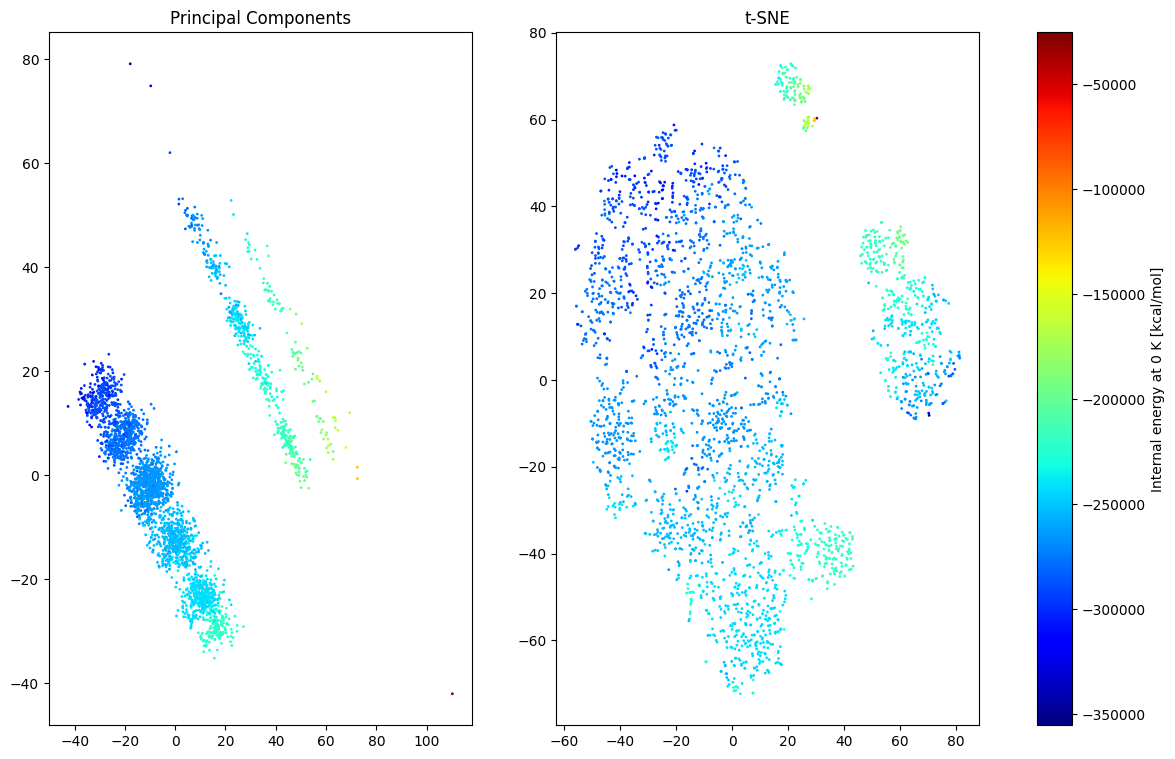
\includegraphics[width=0.9\linewidth]{fig/cm_pca_tsne.png}
    \caption{การกระจายตัวของ Coulomb Matrix Feature ที่ถูกลดจำนวนมิติให้เหลือเพียงแค่ 2 มิติ (Principal Components = 2)}
    \label{fig:cm_pca_tsne}
\end{figure}

โดยเราจะได้พล็อตตามที่ได้ในภาพที่ \ref{fig:cm_pca_tsne} โดยข้อมูลแต่ละจุดนั้นจะถูกไฮไลต์ด้วยสีที่มีสเกลแตกต่างกันไปซึ่งแสดงค่าของพลังงานภายในของโมเลกุล
